\documentclass[11pt]{article}
\usepackage[utf8]{inputenc}
\usepackage{fontspec}
\usepackage{graphicx}
\usepackage{comment}
\usepackage{hyperref}
\usepackage{multirow}
\usepackage{subfigure}
\usepackage{mathtools}


\setmainfont{Times New Roman}
\title{Project \#4}
\author{Riccardo De Zen - 2019295 \\ Mattia Fanan - 2019138 \\ Niccolo' Turcato - 2021446}
\date{a.a. 20/21}

\begin{comment}
	Compile with LuaLatex or xetex
\end{comment}


\addtolength{\oddsidemargin}{-1.5cm}
\addtolength{\evensidemargin}{-1.5cm}
\addtolength{\textwidth}{3cm}
\addtolength{\topmargin}{-1.5cm}
\addtolength{\textheight}{3cm}

\begin{document}
\maketitle
\tableofcontents

\newpage

\section{Introduction}
\input{intro}

\section{Methods}
The implemented methodology follows the BCI literature. \\
Work is divided in two main tasks for each subject: 
\begin{itemize}
\item Creation and calibration of a classifier based on "offline" data
\item Classification of "online" data (serving also as a test)
\end{itemize}\noindent
{\Large \textbf{Data manipulation:}}
The provided data is in the form of raw EEG [samples x channels], and since in this state it is not useful for classifications, we used the procedure described in class to compute the corresponding PSD [windows x frequencies x channels].\\
Before applying the actual PSD procedure, the EEG data is first transformed into the laplacian referencing with a filter [channels x channels] (Figure \ref{fig:laplacian_filter}) in order to enhance the localization of the events related to the executed tasks (Figure \ref{fig:code_raw_eeg_lap}).\\

\begin{figure}[h!]
	\begin{center}
		 \includegraphics[width=0.4\linewidth]{img/code_raw_eeg_lap.PNG}
	\end{center}

	 \caption{load EEG for offline data - compute Laplacian referencing and PSD for one patient}
	 \label{fig:code_raw_eeg_lap}
\end{figure}

\begin{figure}[h!]
	\begin{center}
		 \includegraphics[width=0.5\linewidth]{img/laplacian_filter.png}
	\end{center}

	 \caption{Laplacian filter (16x16)}
	 \label{fig:laplacian_filter}
\end{figure}

After this we splitted the data into the offline part used to train an tuning and the online part used as test.\\ \\
{\Large \textbf{Offline task:}}
\begin{itemize}
\item \textbf{Feature selection:}  For each patient, from the data in form of PSD, then the more discriminant features are selected, each feature corresponds to a (frequency, channel) pair. In this step, we take into account only if the pairs that are meaningful for MI tasks that are the beta
\footnote{for beta rhythm we mean the activity of populations of neurons in the motor-cortex region(also frontal region but is not related to motor-imagery tasks) approximately with frequencies 13-30 (can slightly change from subject to subject)}
 and mu
 \footnote{for mu rhythm we mean the activity of populations of neurons in the motor-cortex region approximately with frequencies 8-13 (can slightly change from subject to subject)}
rhythms.\\
In other words:
\begin{itemize}
\item around the channels C3 and C4 for the task of both hands and around Cz for the task of both feet
\item  in the mu band for the ERD
 \footnote{for ERD -event related de synchronization- we mean when some populations of neurons starts to fire in asynchronous way in response to a task to execute causing a decrease in power of the EEG signal in that area}
 in the beta band for the ERS 
 \footnote{for ERS -event related synchronization- we mean when some populations of neurons after an ERD starts to re-synchronize their firing rate causing an increment in power of the EEG signal in that area}
\end{itemize}
In order to correctly select the most discriminant features we have first normalized the distribution of the samples with respect to the two features we are interested in, applying a logarithmic transformation to the PSD matrix (Figure \ref{fig:freq_data_norm}).
Then we computed the Fisher's score (Figure \ref{fig:fisher_score_calibration_ai6}, Figure \ref{fig:fisher_score_avg_filtered_ai6}) and for removing features that from the literature we know are not related to the tasks, we have applied weights (Figure \ref{fig:features_filter}) to them and then selected the best k (Figure \ref{fig:features_selection}).

\textbf{Choice of k:} We ran a version of subset selection \footnote{Insert Subset selection reference} to choose the optimal number of features for the patients. We used offline data only, so that the results on the online data are as close as possible to a reasonable estimation of the true error of our classifiers, choice of k was in the range [1, 10]. For each patient, we divided the (offline) data in train and validation set (ratios $\frac{2}{3}, \frac{1}{3}$), obtaining the optimal number of features as well as the accuracy on validation data. \\
Then we had to choose if using foreach patient different number of features based on the results obtained as described, or choose k that would be applied to all patients. We went for the second option, as we felt that the tradeoff between optimality and complexity was more reasonable. \\
We computed a weighted average over the patients' results (with the best accuracy as weight) found that about 4 features is probably close to a global optimal number of features for our patients' data.

\begin{figure}[h!]
	\begin{center}
		 \includegraphics[width=0.6\linewidth]{img/code_extract_frequencies_normalize_data.PNG}
	\end{center}

	 \caption{Extracting frequencies, labeling data and normalization}
	 \label{fig:freq_data_norm}
\end{figure}


\begin{figure}[h!]
	\begin{center}
		 \includegraphics[width=0.4\linewidth]{img/features_filter.png}
	\end{center}

	 \caption{Features filter (23x16) (all patients)}
	 \label{fig:features_filter}
\end{figure}

\begin{figure}[h!]
	\begin{center}
		 \includegraphics[width=0.8\linewidth]{img/fisher_score_calibration_ai6.PNG}
	\end{center}

	 \caption{Fisher Score (16x23) (subject ai6)}
	 \label{fig:fisher_score_calibration_ai6}
\end{figure}

\begin{figure}[h!]
	\begin{center}
		 \includegraphics[width=0.8\linewidth]{img/fisher_score_calibration_ai6_avg_filtered.PNG}
	\end{center}

	 \caption{Fisher Score Average on 3 runs and filtered with Features weights (Figure \ref{fig:features_filter}) (16x23) (subject ai6)}
	 \label{fig:fisher_score_avg_filtered_ai6}
\end{figure}



\item \textbf{Classifier training:} The previous steps allow to build a training set for each subject (one can use all the available offline data), by selecting the windows associated with the MI tasks. Then for each subject we applied k-fold cross validation to choose between three differ kind of classificators (LDA, QDA, SVM with rbf kernel). (Figure \ref{fig:cv_ai6})\\

\begin{figure}[h!]
	\begin{center}
		 \includegraphics[width=0.8\linewidth]{img/code_select_features.PNG}
	\end{center}

	 \caption{Features selection}
	 \label{fig:features_selection}


	\begin{center}
		 \includegraphics[width=0.5\linewidth]{img/code_extract_train_set.PNG}
	\end{center}

	 \caption{Training set extraction}
	 \label{fig:train_set_extraction}
\end{figure}

\begin{figure}[h!]
	\begin{center}
		 \includegraphics[width=0.5\linewidth]{img/code_cv_ai6.PNG}
	\end{center}

	 \caption{Results of Cross validation on subject ai6}
	 \label{fig:cv_ai6}
\end{figure}

\begin{figure}[h!]
	\begin{center}
		 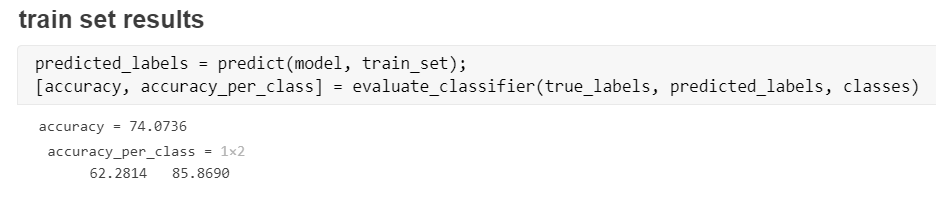
\includegraphics[width=0.7\linewidth]{img/code_train_set_results_ai6.PNG}
	\end{center}

	 \caption{Results of the trained classifier on training data (subject ai6)}
	 \label{fig:train_results_ai6}
\end{figure}


At the end of this step, for each subject we have a trained classifier, that takes in input the selected features from a window of the PSD, and returns in output the label of the MI task that it recognizes. \\
\item \textbf{Evidence accumulation tuning:} We implemented 3 evidence accumulation frameworks, based on different smoothing functions:
	\begin{itemize}
		\item Exponential smoothing: $\Delta_{y_t} = \alpha  (x_t - y_{t-1})$, $y_t = \alpha x_t +(1 - \alpha) y_{t-1}$
		\item Dynamic smoothing: $\Delta_{y_t} = \beta  (\alpha F_{free}(y_{t-1}) + (1 - \alpha) F_{bmi}(x_t))$, $y_t = y_{t-1} + \Delta_{y_t}$
		\item Moving average smoothing: $y_t = \alpha x_t +(1 - \alpha) \frac{\Sigma_{i=1}^{t-1}(y_i) + x_t}{t} $

	\end{itemize}
The last one serves more as a reference for the other two. \\
For each framework we performed parameters' tuning using a genetic algorithm \footnote{Global optimization toolbox (Matlab)}. We performed two different tunings:
	\begin{itemize}
		\item First tuning on the whole offline data, that is then tested on the online data
		\item Second tuning on the first run of online data, that is then tested on the rest of online data
	\end{itemize}
Results are avalaialble in section \ref{sec:results}.
\end{itemize}

\noindent
{\Large\textbf{Online task:}}

\begin{itemize}
\item \textbf{Feature extraction:} Given the online data we extract from it the same features we found in the offline data for the subject (Figure \ref{fig:load_online_data_classifier_features_extraction}). 

\begin{figure}[h!]
	\begin{center}
		 \includegraphics[width=0.7\linewidth]{img/code_load_online_and_features_extraction.PNG}
	\end{center}

	 \caption{Load of online data, trained classifier (for current subject), features  extraction}
	 \label{fig:load_online_data_classifier_features_extraction}
\end{figure}



\item \textbf{Classification test:} Once we have extracted the features, the classifier trained for the current patient is used to estimate the performed task, with a certain confidence value (Figure \ref{fig:test_results_ai6}). \\

\begin{figure}[h!]
	\begin{center}
		 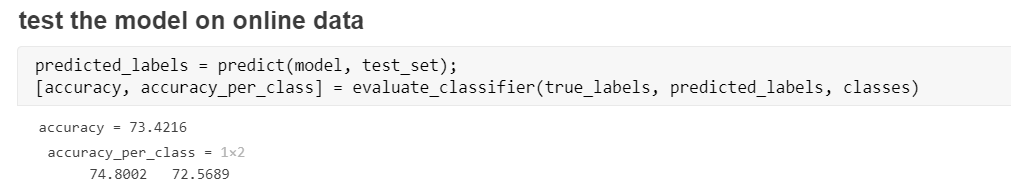
\includegraphics[width=0.7\linewidth]{img/code_test_set_results_ai6.PNG}
	\end{center}

	 \caption{Results of the trained classifier on test data (subject ai6)}
	 \label{fig:test_results_ai6}
\end{figure}

At last, we can evaluate the performance of the system with single-sample accuracy.
\item \textbf{Evidence accumulation test:} Then we used the evidence accumulation frameworks (with the parameters found in the tuning sessions for the subject) over the predictions of the classifier.\\
At the end we evaluate the performance on the continuos feedback period in order to obtain a trial level accuracy.
\end{itemize}

\section{Results}
\label{sec:results}

\begin{figure}
    \begin{center}
        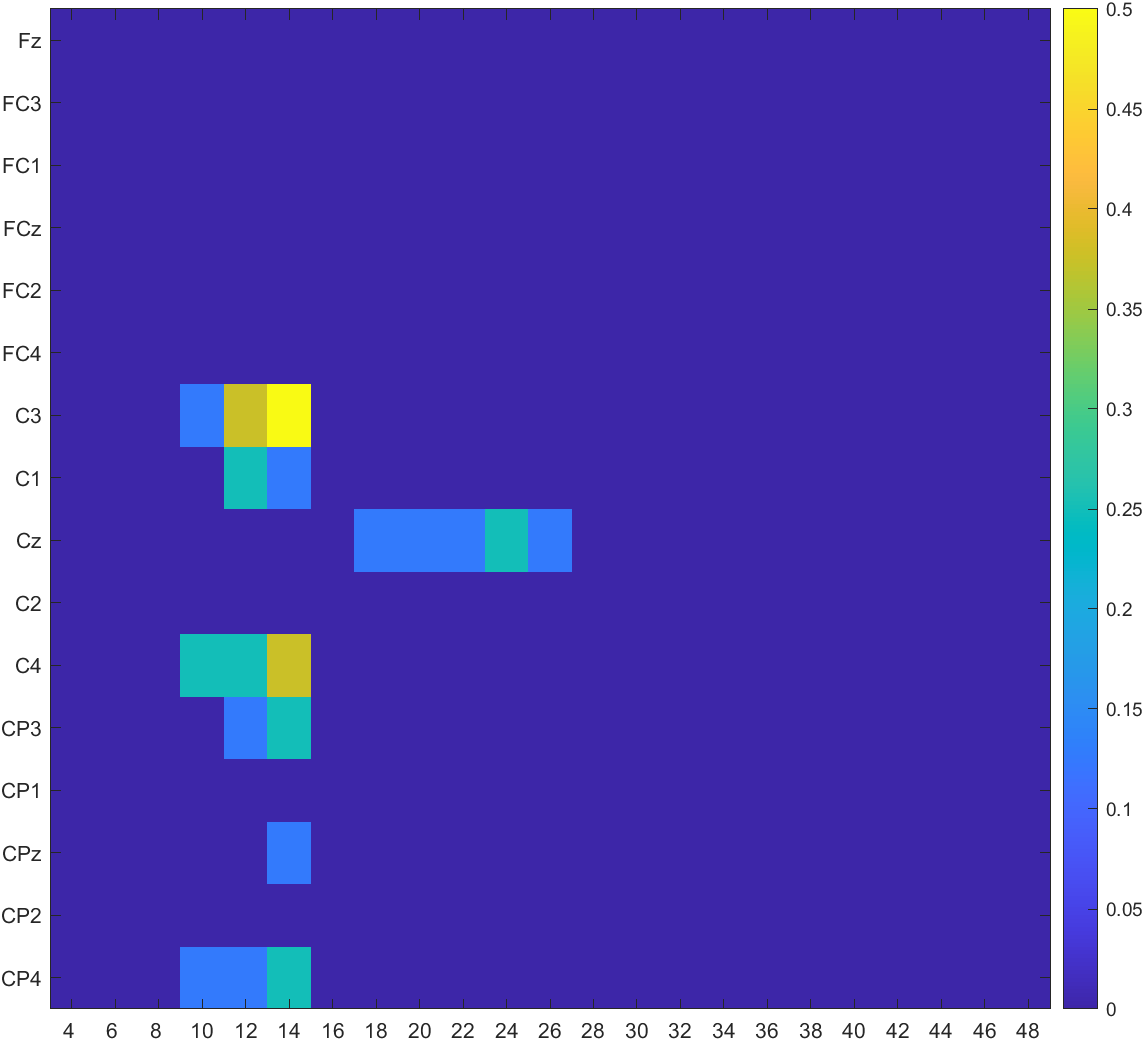
\includegraphics[width=0.5\linewidth]{img/avg_selected_feature_n4features_autofilter.png}
    \end{center}

    \caption{Statistics of features selected over the patients}
    \label{fig:/avg_selected_feature_n4features_autofilter}
\end{figure}

\begin{figure}

\begin{center}
      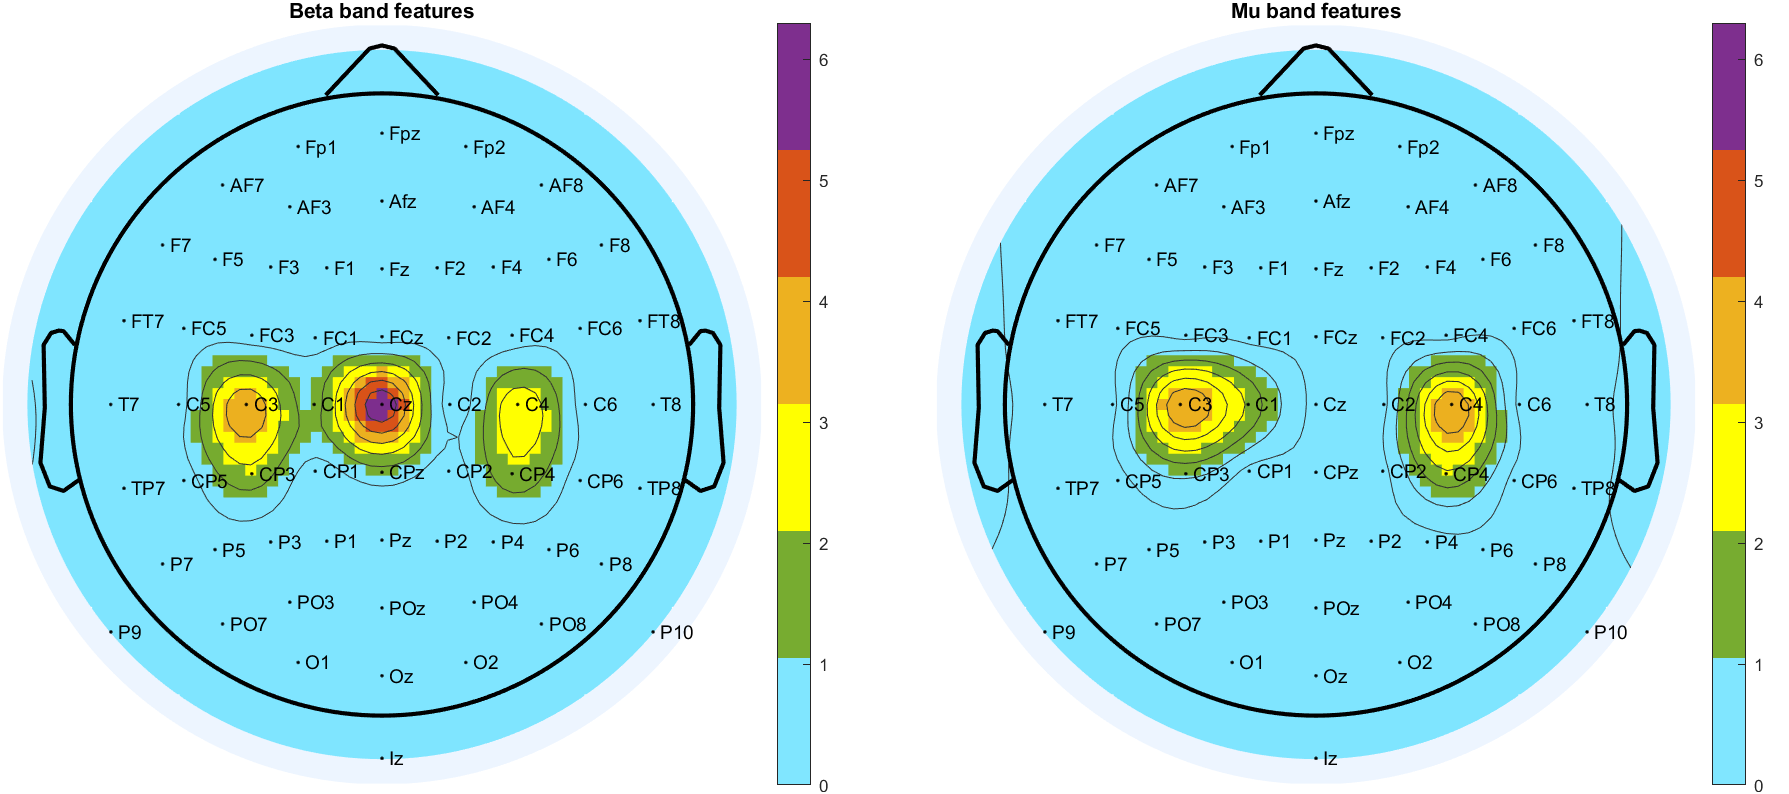
\includegraphics[width=0.6\linewidth]{img/topoplot_electrodes_sel_features_beta_mu_band_n4features_64channelsmap.png}
\end{center}

    \caption{Number og features selected for each electrode over the patients}
    \label{fig:/avg_selected_feature_per_electrode_n4features_autofilter_channels64}
\end{figure}


\begin{tabular}{||c|c|c|c|c|c|c||}
    \hline
    \multicolumn{7}{||c||}{Single Sample accuracy}                                                 \\
    \hline
    \multirow{2}{*}{Patient} &
    \multicolumn{3}{|c|}
    {Single sample offline}  &
    \multicolumn{3}{|c||}
    {Single sample online}                                                                         \\
    \cline{2-7}
    % --
                             & Average & Both Feet & Both Hands & Average & Both Feet & Both Hands \\
    \hline\hline
    ai6                      & 75,85   & 66,92     & 84,79      & 67,57   & 69,44     & 65,99      \\
    ai7                      & 85,12   & 83,06     & 87,18      & 76,33   & 75,65     & 76,97      \\
    ai8                      & 83,89   & 80,36     & 87,43      & 71,62   & 62,52     & 82,40      \\
    aj1                      & 90,70   & 92,30     & 89,09      & 74,31   & 76,53     & 72,74      \\
    aj3                      & 85,19   & 85,29     & 85,09      & 77,04   & 70,52     & 85,55      \\
    aj4                      & 77,08   & 68,54     & 85,62      & 70,81   & 76,57     & 65,96      \\
    aj7                      & 73,52   & 72,79     & 74,24      & 59,58   & 32,48     & 83,02      \\
    aj9                      & 80,62   & 77,10     & 84,14      & 68,48   & 53,84     & 78,72      \\
\hline
    AVG                      & 81,50   & 78,29     & 84,70      & 70,72   & 64,69     & 76,42      \\
    \hline
\end{tabular}

\begin{tabular}{||c|c|c|c|c|c|c|c||}
    \hline
    \multicolumn{8}{||c||}{Moving Average (offline tuning)}                                                   \\
    \hline
    \multirow{2}{*}{Patient} &
    \multicolumn{2}{|c|}
    {Offline data}           &
    \multicolumn{2}{|c|}
    {Online data}            &
    \multicolumn{3}{|c||}
    {Parameters}                                                                                              \\
    \cline{2-8}
    % --
                             & $P_{act}$ & $P_{rej}$ & $P_{act}$ & $P_{rej}$ & $\alpha$ & $t_{BH}$ & $t_{BF}$ \\
    \hline\hline
    ai6                      & 85,56     & 85,56     & 53,33     & 58,72     & 0,87     & 0,87     & 0,23     \\
    ai7                      & 95,56     & 95,56     & 76,67     & 85,98     & 0,77     & 0,83     & 0,13     \\
    ai8                      & 96,67     & 96,67     & 79,17     & 81,90     & 0,78     & 0,79     & 0,14     \\
    aj1                      & 95,00     & 96,61     & 81,67     & 85,22     & 0,60     & 0,85     & 0,11     \\
    aj3                      & 91,11     & 92,13     & 81,67     & 87,50     & 0,58     & 0,63     & 0,13     \\
    aj4                      & 92,22     & 92,22     & 66,67     & 76,92     & 0,96     & 0,90     & 0,22     \\
    aj7                      & 86,67     & 89,66     & 52,50     & 56,25     & 0,97     & 0,84     & 0,17     \\
    aj9                      & 95,56     & 98,85     & 49,17     & 71,08     & 0,90     & 0,87     & 0,17     \\
\hline
    AVG                      & 92,29     & 93,41     & 67,60     & 75,45     & 0,80     & 0,82     & 0,16     \\
    \hline
\end{tabular}

\begin{tabular}{||c|c|c|c|c|c|c|c||}
    \hline
    \multicolumn{8}{||c||}{Moving Average (first online run tuning)}                                          \\
    \hline
    \multirow{2}{*}{Patient} &
    \multicolumn{2}{|c|}
    {Train data (run 1)}     &
    \multicolumn{2}{|c|}
    {Test data (run 2+)}     &
    \multicolumn{3}{|c||}
    {Parameters}                                                                                              \\
    \cline{2-8}
    % --
                             & $P_{act}$ & $P_{rej}$ & $P_{act}$ & $P_{rej}$ & $\alpha$ & $t_{BH}$ & $t_{BF}$ \\
    \hline\hline
    ai6                      & 75,00     & 75,00     & 54,00     & 59,34     & 0,86     & 0,88     & 0,24     \\
    ai7                      & 90,00     & 94,74     & 81,00     & 86,17     & 0,76     & 0,85     & 0,13     \\
    ai8                      & 85,00     & 85,00     & 78,00     & 78,00     & 0,51     & 0,64     & 0,20     \\
    aj1                      & 95,00     & 95,00     & 80,00     & 80,00     & 0,69     & 0,77     & 0,10     \\
    aj3                      & 95,00     & 95,00     & 85,00     & 88,54     & 0,70     & 0,84     & 0,14     \\
    aj4                      & 90,00     & 90,00     & 62,00     & 65,26     & 0,64     & 0,76     & 0,26     \\
    aj7                      & 70,00     & 87,50     & 28,00     & 68,29     & 0,64     & 0,70     & 0,17     \\
    aj9                      & 95,00     & 100,00    & 46,00     & 64,79     & 0,86     & 0,83     & 0,17     \\
\hline
    AVG                      & 86,88     & 90,28     & 64,25     & 73,80     & 0,71     & 0,78     & 0,18     \\
    \hline
\end{tabular}

\begin{tabular}{||c|c|c|c|c|c|c|c||}
    \hline
    \multicolumn{8}{||c||}{Exponential Smoothing (offline tuning)}                                            \\
    \hline
    \multirow{2}{*}{Patient} &
    \multicolumn{2}{|c|}
    {Offline data}           &
    \multicolumn{2}{|c|}
    {Online data}            &
    \multicolumn{3}{|c||}
    {Parameters}                                                                                              \\
    \cline{2-8}
    % --
                             & $P_{act}$ & $P_{rej}$ & $P_{act}$ & $P_{rej}$ & $\alpha$ & $t_{BH}$ & $t_{BF}$ \\
    \hline\hline
    ai6                      & 91,11     & 94,25     & 80,83     & 88,99     & 0,96     & 0,66     & 0,40     \\
    ai7                      & 100,00    & 100,00    & 93,33     & 93,33     & 0,88     & 0,72     & 0,19     \\
    ai8                      & 100,00    & 100,00    & 84,17     & 84,17     & 0,72     & 0,85     & 0,18     \\
    aj1                      & 100,00    & 100,00    & 82,50     & 86,84     & 0,70     & 0,92     & 0,06     \\
    aj3                      & 100,00    & 100,00    & 95,83     & 98,29     & 0,91     & 0,74     & 0,16     \\
    aj4                      & 96,67     & 97,75     & 75,00     & 78,95     & 0,92     & 0,68     & 0,31     \\
    aj7                      & 91,67     & 93,22     & 55,83     & 57,76     & 0,59     & 0,78     & 0,22     \\
    aj9                      & 100,00    & 100,00    & 65,83     & 84,04     & 0,94     & 0,71     & 0,34     \\
\hline
    AVG                      & 97,43     & 98,15     & 79,17     & 84,05     & 0,83     & 0,76     & 0,23     \\
    \hline
\end{tabular}

\begin{tabular}{||c|c|c|c|c|c|c|c||}
    \hline
    \multicolumn{8}{||c||}{Exponential Smoothing (first online run tuning)}                                   \\
    \hline
    \multirow{2}{*}{Patient} &
    \multicolumn{2}{|c|}
    {Train data (run 1)}     &
    \multicolumn{2}{|c|}
    {Test data (run 2+)}     &
    \multicolumn{3}{|c||}
    {Parameters}                                                                                              \\
    \cline{2-8}
    % --
                             & $P_{act}$ & $P_{rej}$ & $P_{act}$ & $P_{rej}$ & $\alpha$ & $t_{BH}$ & $t_{BF}$ \\
    \hline\hline
    ai6                      & 95,00     & 95,00     & 75,00     & 90,36     & 0,80     & 0,87     & 0,28     \\
    ai7                      & 95,00     & 95,00     & 95,00     & 95,00     & 0,87     & 0,76     & 0,20     \\
    ai8                      & 90,00     & 90,00     & 93,00     & 93,00     & 0,92     & 0,58     & 0,28     \\
    aj1                      & 100,00    & 100,00    & 92,00     & 92,00     & 0,86     & 0,79     & 0,08     \\
    aj3                      & 100,00    & 100,00    & 93,00     & 93,00     & 0,81     & 0,84     & 0,23     \\
    aj4                      & 95,00     & 100,00    & 74,00     & 81,32     & 0,99     & 0,60     & 0,40     \\
    aj7                      & 80,00     & 94,12     & 21,00     & 67,74     & 0,18     & 0,85     & 0,11     \\
    aj9                      & 100,00    & 100,00    & 58,00     & 79,45     & 0,91     & 0,78     & 0,29     \\
\hline
    AVG                      & 94,38     & 96,76     & 75,13     & 86,48     & 0,79     & 0,76     & 0,23     \\
    \hline
\end{tabular}

\begin{tabular}{||c|c|c|c|c|c|c|c|c|c|c||}
    \hline
    \multicolumn{11}{||c||}{Dynamic Force (offline tuning)}                                                                                   \\
    \hline
    \multirow{2}{*}{Patient} &
    \multicolumn{2}{|c|}
    {Offline data}           &
    \multicolumn{2}{|c|}
    {Online data}            &
    \multicolumn{6}{|c||}
    {Parameters}                                                                                                                              \\
    \cline{2-11}
    % --
                             & $P_{act}$ & $P_{rej}$ & $P_{act}$ & $P_{rej}$ & $\alpha$ & $\beta$ & $\sigma$ & $\omega$ & $t_{BH}$ & $t_{BF}$ \\
    \hline\hline
    ai6                      & 91,11     & 94,25     & 74,17     & 81,65     & 0,06     & 0,06    & 0,37     & 0,45     & 0,82     & 0,38     \\
    ai7                      & 100,00    & 100,00    & 93,33     & 95,73     & 0,57     & 0,13    & 0,20     & 0,24     & 0,76     & 0,13     \\
    ai8                      & 100,00    & 100,00    & 90,00     & 90,00     & 0,22     & 0,13    & 0,41     & 0,42     & 0,96     & 0,13     \\
    aj1                      & 100,00    & 100,00    & 85,83     & 85,83     & 0,02     & 0,03    & 0,05     & 0,12     & 0,75     & 0,30     \\
    aj3                      & 100,00    & 100,00    & 98,33     & 100,00    & 0,67     & 0,18    & 0,15     & 0,24     & 0,82     & 0,30     \\
    aj4                      & 96,67     & 96,67     & 70,83     & 76,58     & 0,29     & 0,29    & 0,30     & 0,39     & 0,91     & 0,24     \\
    aj7                      & 95,00     & 95,00     & 57,50     & 58,47     & 0,55     & 0,70    & 0,08     & 0,40     & 0,85     & 0,16     \\
    aj9                      & 100,00    & 100,00    & 64,17     & 89,53     & 0,15     & 0,11    & 0,58     & 0,44     & 0,97     & 0,15     \\
\hline
    AVG                      & 97,85     & 98,24     & 79,27     & 84,72     & 0,32     & 0,20    & 0,27     & 0,34     & 0,85     & 0,22     \\
    \hline
\end{tabular}

\begin{tabular}{||c|c|c|c|c|c|c|c|c|c|c||}
    \hline
    \multicolumn{11}{||c||}{Dynamic Force (first online run tuning)}                                                                          \\
    \hline
    \multirow{2}{*}{Patient} &
    \multicolumn{2}{|c|}
    {Train data (run 1)}     &
    \multicolumn{2}{|c|}
    {Test data (run 2+)}     &
    \multicolumn{6}{|c||}
    {Parameters}                                                                                                                              \\
    \cline{2-11}
    % --
                             & $P_{act}$ & $P_{rej}$ & $P_{act}$ & $P_{rej}$ & $\alpha$ & $\beta$ & $\sigma$ & $\omega$ & $t_{BH}$ & $t_{BF}$ \\
    \hline\hline
    ai6                      & 95,00     & 95,00     & 69,00     & 92,00     & 0,52     & 0,15    & 0,33     & 0,40     & 0,94     & 0,44     \\
    ai7                      & 95,00     & 100,00    & 72,00     & 86,75     & 0,41     & 0,17    & 0,80     & 0,06     & 0,62     & 0,28     \\
    ai8                      & 90,00     & 90,00     & 87,00     & 87,00     & 0,03     & 0,09    & 0,58     & 0,35     & 0,56     & 0,19     \\
    aj1                      & 100,00    & 100,00    & 92,00     & 92,00     & 0,22     & 0,03    & 0,63     & 0,13     & 0,55     & 0,13     \\
    aj3                      & 100,00    & 100,00    & 91,00     & 91,00     & 0,63     & 0,20    & 0,21     & 0,10     & 0,93     & 0,37     \\
    aj4                      & 100,00    & 100,00    & 59,00     & 59,00     & 0,67     & 0,09    & 0,51     & 0,01     & 0,73     & 0,24     \\
    aj7                      & 95,00     & 100,00    & 47,00     & 64,38     & 0,54     & 0,34    & 0,17     & 0,31     & 0,70     & 0,03     \\
    aj9                      & 100,00    & 100,00    & 49,00     & 84,48     & 0,04     & 0,05    & 0,45     & 0,09     & 0,98     & 0,26     \\
\hline
    AVG                      & 96,88     & 98,13     & 70,75     & 82,08     & 0,38     & 0,14    & 0,46     & 0,18     & 0,75     & 0,24     \\
    \hline
\end{tabular}


\begin{figure}
    \begin{center}
        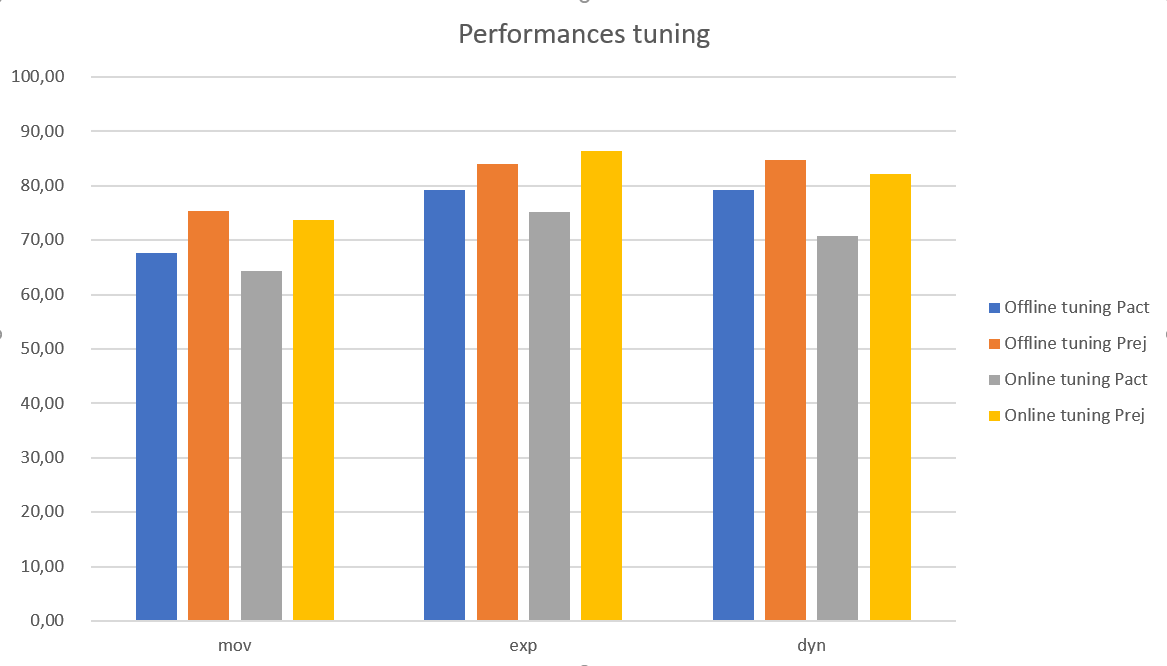
\includegraphics[width=0.8\linewidth]{img/tunings_performances.png}
    \end{center}

    \caption{Comparison of tuning on offline vs tuning on online data (AVG results)}
    \label{fig:/comparison_tunings}
\end{figure}


\section{Discussion}
First thing, we notice that our results are aligned with the reference results, both in terms of single sample and evidence accumulation accuracy, feature selection and choice of parameters. \\
It's no surprise that the chosen electrodes are over the central area of the cortex, indicating that the subjects of the study, overall were able to correctly modulate their brain activity for the MI tasks. Moverover, this also indicates that the data analysis and manipulation is working correctly.\\
We would like to remark that the use of a features filter (Figure \ref{fig:features_filter}) has allowed to basically automate the whole process, whitout the need to manually control features for each subject. \\

As expected, results are really dependent on the single subject, and while in average the results are good, it is easy to see that a subset of patients performs poorly, while the rest in general has excellent performance. \\
There could be room for improvement though, using different spatial filters for the subset of poorly-performant subjects, as the literature (ref PAPER spatial filters) shows that there are available other s. filters that give better results than (small) laplatian. \\

As one could have anticipated, single sample results are mediocre, though they are far from bein random. 
Again, not contradicting our expectations, ev.acc. framework do improve considerably our results confirming that the classifiers did infact learn to recognize MI tasks.

Contrary to our expectation, the data was lacking resting trials, both in the offline and online data, for every patient, this has probably resulted in a benefit for our classification results with the evidence accumulation frameworks. The optimization algorithm has computed more restricting thresholds, in order to exploit the classificators' output, resulting in a more precise trial level classification.

To analize evidence accumulation performance, we computed both accuracy over correctly classified trials and over correctly classified trials not considering trials that the framework could not classify (the curve does not cross any threshold).

Of the 3 control frameworks, both exponential and dynamic smoothing obtain reasonable results, while the one based on moving average falls behind current state of the art performances.

Of the two parameters' tuning techniques there is not a clear winner, if we were to consider only performance with rejection, we would say that exponential smoothing tuned over the first online run works best. If, instead, we were to consider only performance without rejection, we would probably choose that dynamic smoothing tuned over offline data. \\

While online tuning does not produce encouraging results in this case, we must also consider that this technique uses considerably less data than the offline tuning, therefore it's very likely that if we had more online runs available, we could have obtained more satisfying performances.









\end{document}